 \iffalse
\let\negmedspace\undefined
\let\negthickspace\undefined
\documentclass[journal,12pt,twocolumn]{IEEEtran}
\usepackage{xparse}
\usepackage{cite}
\usepackage{amsmath,amssymb,amsfonts,amsthm}
\usepackage{algorithmic}
\usepackage{graphicx}
\usepackage{textcomp}
\usepackage{xcolor}
\usepackage{txfonts}
\usepackage{listings}
\usepackage{enumitem}
\usepackage{mathtools}
\usepackage{gensymb}
\usepackage{comment}
\usepackage[breaklinks=true]{hyperref}
\usepackage{tkz-euclide} 
\usepackage{listings}
\usepackage{gvv}                                        
\def\inputGnumericTable{}                                 
\usepackage[latin1]{inputenc}                                
\usepackage{color}                                            
\usepackage{array}                                            
\usepackage{longtable}                                       
\usepackage{calc}                                             
\usepackage{multirow}                                         
\usepackage{hhline}                                           
\usepackage{ifthen}                                           
\usepackage{lscape}

\newtheorem{theorem}{Theorem}[section]
\newtheorem{problem}{Problem}
\newtheorem{proposition}{Proposition}[section]
\newtheorem{lemma}{Lemma}[section]
\newtheorem{corollary}[theorem]{Corollary}
\newtheorem{example}{Example}[section]
\newtheorem{definition}[problem]{Definition}
\newcommand{\BEQA}{\begin{eqnarray}}
\newcommand{\EEQA}{\end{eqnarray}}
\newcommand{\define}{\stackrel{\triangle}{=}}
\theoremstyle{remark}
\newtheorem{rem}{Remark}
\begin{document}

\bibliographystyle{IEEEtran}
\vspace{3cm}

\title{GATE-CS.51}
\author{EE23BTECH11046 - Poluri Hemanth$^{*}$}
\maketitle
\textbf{Question:}
Consider the following recurrence:
\begin{align}
	f(1)\;\;&=\;\;1;\label{g2-1cs.51}\\
	 f(2n)\;\;&=\;2f(n)-1,\text{  for $n\geq$1;}\label{g2-2cs.51}\\
	 f(2n+1)\;\;&=\;2f(n)+1,\text{  for $n\geq$1.}\label{g2-3cs.51}
\end{align}
Then, which of thefollowing is/are \textbf{TRUE?}\\
(A) $f(2^n-1)\;=\;2^n-1$\\
(B) $f(2^n)\;=\;1$\\
(C) $f(5\cdot2^n)\;=\;2^{n+1}+1$\\
(D) $f(2^n+1)\;=\;2^n+1$\\
\hfill{[GATE-CS.51 2022]}\\
\textbf{Solution:}\\
\fi
(A)\\
let $x(2^k-1)=2^k-1$ for any $k\geq1$,
\begin{align}
	x(2^{k+1}-1)&=x(2(2^k-1)+1)
\end{align}
From \eqref{g2-3cs.51},
\begin{align}
	&=2x(2^k-1)+1\\
        &=2(2^k-1)+1\\
	&=2^{k+1}-1\label{1.cs51}
\end{align}
From \eqref{g2-1cs.51},\eqref{1.cs51}
\begin{align}
	x(2-1)&=2-1\text{  ($k=0$)}\\
	&=1
\end{align}
Hence $x(2^n-1)=2^n-1$ for $n\geq1$\\
So statement A is TRUE\\
\\(B)\\
Let $x(2^k)=1$ for any $k\geq$0
\begin{align}
	x(2^{k+1})&=x(2\cdot2^k)
\end{align}
From \eqref{g2-2cs.51}
\begin{align}
	&=2x(2^k)-1\label{2cs.51}\\
	&=1
\end{align}
From \eqref{2cs.51},\eqref{g2-2cs.51}
\begin{align}
	x(2)&=2x(1)-1\\
	&=1\label{bcs.51}
\end{align}
Hence $x(2^n)=1$ for every $n\geq0$ value.\\
So statement B is TRUE.\\
\\(C)\\
Let,$x(5\cdot2^k)=2^{k+1}+1$ be true for any $k\geq0$,
\begin{align}
	x(5\cdot2^{k+1})&=x(2(5\cdot2^k))
\end{align}
From \eqref{g2-2cs.51}
\begin{align}
	&=2x(5\cdot2^k)-1\\
	&=2^{k+2}+1\label{3cs.51}
\end{align}
$k=-1$ ,From \eqref{3cs.51}
\begin{align}
	x(5)&=2^1+1\\
	&=3
\end{align}
Proof:-
\begin{align}
        x(5)&=x(2\cdot2+1)
\end{align}
From \eqref{g2-3cs.51},\eqref{bcs.51}
\begin{align}
        &=2x(2)+1\\
        &=3
\end{align}
Hence $x(5.2^n)=2^{n+1}+1$ for $n\geq1$\\
So statement C is TRUE.\\
\\(D)
\begin{align}
	x(2^n+1)&=x(2\cdot2^{n-1}+1)
\end{align}
From \eqref{g2-3cs.51},\eqref{bcs.51}
\begin{align}
	&=2x(2^{n-1})+1\\
	&=3
\end{align}
Hence statement D is FALSE.
\begin{figure}
	\centering
	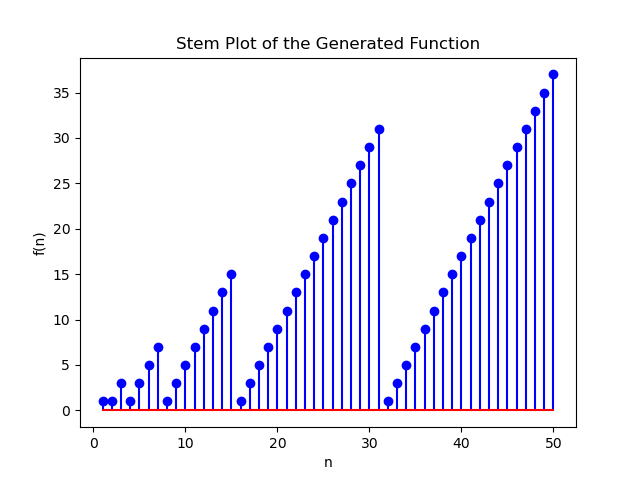
\includegraphics[width=1\columnwidth]{2022/CS/51/figures/gate2.png}
	\caption{plot of $x(n)$}
	\label{cs.51.stem}
\end{figure}







%\end{document}
